\documentclass[11pt]{article}
\usepackage{latexsym}
\usepackage{amsmath}
\usepackage{amssymb}
\usepackage{amsthm}
\usepackage{epsfig}
\usepackage[tight]{subfigure}

\usepackage{amsmath}

\DeclareMathOperator*{\minimize}{min}
\DeclareMathOperator*{\maximize}{max}

\usepackage{algorithm}
 %on linux you may need to run sudo apt-get install texlive-full to install algorithm.sys
\usepackage{algorithmic}

\usepackage{verbatim}

\newcommand{\handout}[5]{
  \noindent
  \begin{center}
  \framebox{
    \vbox{
      \hbox to 5.78in { {#1} \hfill #2 }
      \vspace{4mm}
      \hbox to 5.78in { {\Large \hfill #5  \hfill} }
      \vspace{2mm}
      \hbox to 5.78in { {\em #3 \hfill #4} }
    }
  }
  \end{center}
  \vspace*{4mm}
}

\newcommand{\lecture}[5]{\handout{#1}{#2}{#3}{#4}{#5}}
\newcommand{\collision}[0]{\mathrm{collision}}
\newcommand{\nocollision}[0]{\overline{\collision}}

\newcommand*{\QED}{\hfill\ensuremath{\square}}

\newtheorem{theorem}{Theorem}
\newtheorem{corollary}[theorem]{Corollary}
\newtheorem{lemma}[theorem]{Lemma}
\newtheorem{observation}[theorem]{Observation}
\newtheorem{proposition}[theorem]{Proposition}
\newtheorem{definition}[theorem]{Definition}
\newtheorem{claim}[theorem]{Claim}
\newtheorem{fact}[theorem]{Fact}
\newtheorem{assumption}[theorem]{Assumption}
\newtheorem{note}[theorem]{Note}


\newcommand{\norm}[1]{\left\lVert#1\right\rVert}
\usepackage{bbm}



% 1-inch margins, from fullpage.sty by H.Partl, Version 2, Dec. 15, 1988.
\topmargin 0pt
\advance \topmargin by -\headheight
\advance \topmargin by -\headsep
\textheight 8.9in
\oddsidemargin 0pt
\evensidemargin \oddsidemargin
\marginparwidth 0.5in
\textwidth 6.5in

\parindent 0in
\parskip 1.5ex
%\renewcommand{\baselinestretch}{1.25}

\begin{document}

\lecture{Statistical Techniques in Robotics (16-831, S20)}{Lecture \#17
  (Wednesday, April 7)}{Lecturer: Kris Kitani}{Scribes: Tanay Sharma, Paritosh Mittal}{Model-Free Value Prediction}

\section{Review}
In the last lecture, on the topic of Value Based Reinforcement Learning (RL) algorithms, we learned Value functions and their recurrent relationship was stated using Bellman Equations. The Value Based RL paradigm can be understood by Fig 1. Since we explicitly estimate value functions to estimate the best policy, these methods are termed as Value Based. There are mainly two types of algorithms under this (1) Model-Based algorithms (2) Model-Free Algorithms. We studied about Model Based algorithms. It means that the model is fully specified and we have the transition dynamics and reward function already. Under model based methods we learned two algorithms (1) Policy Iteration (2) Value Iteration.

\begin{center}
    \begin{figure}[h]
        \centering
        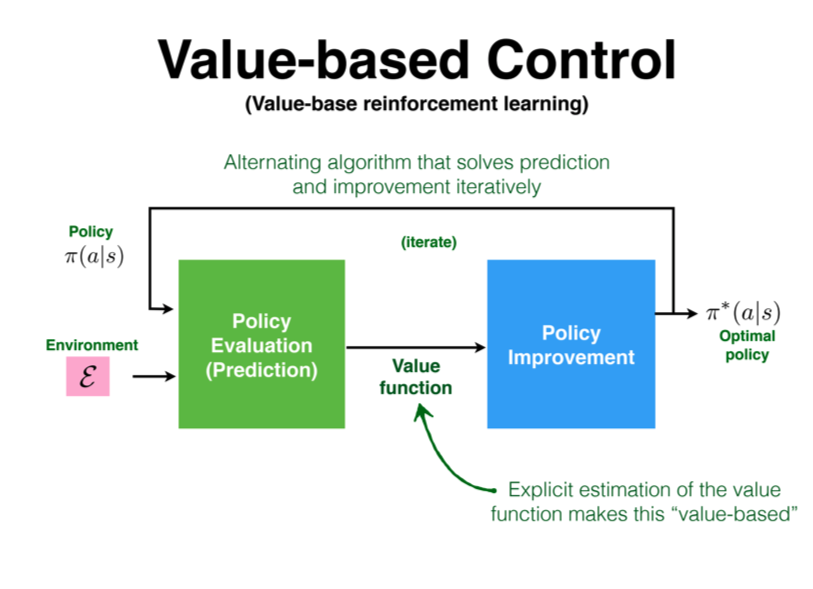
\includegraphics[width=0.6\textwidth]{images/ValueBased.png}
        \caption{Caption}
        \label{fig:my_label}
    \end{figure}
\end{center}

\subsection{Policy Iteration}
To understand this algorithm we recall the Bellman Equations which are given as :

\begin{equation}
\begin{array}{c}
V^{\pi}(s)=\sum_{a} \pi(a \mid s) \sum_{s^{\prime}} p\left(s^{\prime} \mid s, a\right)\left[r\left(s^{\prime}, a, s\right)+\gamma V^{\pi}\left(s^{\prime}\right)\right] \\
Q^{\pi}(s, a)=\sum_{s^{\prime}} p\left(s^{\prime} \mid s, a\right)\left\{r\left(s^{\prime}, a, s\right)+\sum_{a^{\prime}} \pi\left(a^{\prime} \mid s^{\prime}\right) Q^{\pi}\left(s^{\prime}, a^{\prime}\right)\right\}
\end{array}
\end{equation}

Policy iteration builds on this recursive algorithm that we know needs to be satisfied. As can be seen in Fig 1, there are two steps in value based control algorithms (1) Policy Evaluation (Prediction) (2) Policy Improvement. \\
The algorithm for policy iteration is shown below : \\

\begin{algorithm}[H]
\caption{POLICY\_ITERATION $\left(\pi, r(s), p\left(s^{\prime} \mid s, a\right), \gamma\right)$}
\label{algo:wma}
\begin{algorithmic}[1]
\STATE $\pi \leftarrow \operatorname{rand}(\mathcal{A})$
\STATE $V \leftarrow \operatorname{rand}(\mathbb{R})$
\STATE $V^{\prime} \leftarrow \operatorname{rand}(\mathbb{R})$
\WHILE {$\max _{s}\left|V(s)-V^{\prime}(s)\right| \geq \epsilon$}
\STATE \qquad $V^{\prime} \leftarrow V$
\FOR{$s \in \mathcal{S}$}
\STATE $Q(s, a)=r(s)+\gamma \sum_{s^{\prime}} p\left(s^{\prime} \mid s, a\right) V^{\prime}\left(s^{\prime}\right) \quad \forall a $
\STATE $V(s)=\sum_{a} \pi(a \mid s) Q(s, a)$
\ENDFOR
\ENDWHILE
\FOR {$s \in \mathcal{S}$}
\STATE $\pi^{\prime}(s)=\arg \max _{a} Q(s, a)$
\ENDFOR \\
\IF{$\pi^{\prime}=\pi$}
\STATE \text{return} $\pi$
\ENDIF \\
\text{Go to line 1}
\end{algorithmic}
\end{algorithm}

According to the algorithm, policy evaluation is done from line 6 to 8. We calculate the new estimate of our value function given a policy using the current estimate and update the current estimate with it. We continue this process until the change in consecutive value is below a certain threshold (convergence). Once we have the optimum values of our value function for given policy we go to the policy improvement stage. We know that when the policy is optimal it will be equal to max(Q Value function) (line 11-13). Now the whole process is repeated until our policy converges to an optimal value

\subsection{Value iteration}
Value iteration is a modification of Policy iteration to make the algorithm faster. As policy was updated after value function converges in policy iteration, it takes a lot of time for policy to converge. Value iteration does the policy improvement in the while loop after policy evaluation at each step (after line 8 above). This leads to faster convergence


\section{Model Free Algorithms}
Now we will look into Model Free Algorithms that are another set of algorithms for Value based RL. Unlike model based algorithms, we do no have direct access to the model. Hence, we do not have the transition dynamics and reward function. The only way to calculate the value function to find the optimal policy is by interacting with environment. We can generate many samples by this interaction and samples that we receive can be in the form :
\begin{align}
    \{s^{'}, r, s, a\}_{1}^N
\end{align}
where \(s^{'}\) = new state, \(r\) = reward, \(s\) = current state, \(a\) = action taken, N = number of samples
These types of algorithms are useful in many real-life scenarios where possible states can be huge. In such scenarios, calculating model parameters like transition dynamics and reward function may be tedious, prone to errors or not possible. 
There are two methods mainly to calculate the value function from this sampled interaction with the environment.
\begin{enumerate}
    \item \textbf{System Identification (“Model-based RL”):} In this method we collect many samples from the environment by interaction and convert the model free problem to model based problem by using the samples as data/knowledge about the environment. Once we parameterize the transition dynamics and reward function, we can use the algorithms as described above.
    \item \textbf{Model-free Prediction:} Under these methods , we directly estimate the value function while interacting with the environment. We will look into two categories of such algorithms :
        \begin{enumerate}
            \item Monte Carlo
            \item Temporal Differencing
        \end{enumerate}
\end{enumerate}

\subsection{Monte Carlo Prediction}
Value of a state is the expected (mean) return under the MDP (policy, dynamics, initial state distribution
$$
\begin{aligned}
V^{\pi}(s) &=\mathbb{E}_{\pi, P}\left[\sum_{t=0}^{T} \gamma^{t} r_{t} \mid s_{0}=s\right] \\
&=\mathbb{E}_{\pi, P}\left[G \mid s_{0}=s\right]
\end{aligned}
$$
We cannot calculate this quantity directly in model-free method as we do not have access to transition dynamics. Monte Carlo method estimates the value function by interacting with the environment many times and using the average return value as the value function at that step.
\begin{align}
     V(s) = \frac{1}{N }\sum_{i=1}^N G_i(s)
\end{align}
where \(G_i(s)\) is the total reward at a time step (iteration) i and N is the total number of interactions with the environment starting from state s. 
There are different variants of Monte Carlo estimation methods :
\begin{enumerate}
    \item FirstVisit-MC-Prediction
    \item FirstVisit-Incremental-MC-Prediction
    \item FirstVisit-Dynamic-MC-Prediction
    \item EveryVisit-MC-Prediction
\end{enumerate}

Let us discuss each algorithm independently,
\subsubsection* {First Visit MC Prediction}
\begin{algorithm}[H]
\caption{FIRSTVISIT-MC-PREDICTION $(\pi)$}
\label{algo:fvmcp}
\begin{algorithmic}[1]
\FOR {$e=1, \ldots, E$}
\STATE $\left\{s^{(t)}, a^{(t)}, r^{(t)}\right\}_{t=0}^{T} \sim \mathcal{E} \mid \pi$
\FOR {$t=0, \ldots, T$}
\IF {$\text{first visit to } s^{(t)} \text{ in episode } e$}
\STATE $G\left(s^{(t)}\right) \leftarrow G\left(s^{(t)}\right)+\sum_{i=t}^{T} r^{(i)}$
\STATE $N\left(s^{(t)}\right) \leftarrow N\left(s^{(t)}\right)+1$
\ENDIF
\ENDFOR
\ENDFOR
\STATE $\text{return } V(s) \leftarrow G(s) / N(s) \forall s$
\end{algorithmic}
\end{algorithm}
Key points for First Visit Monte Carlo Prediction:
\begin{itemize}
    \item Line 2: of algo. \ref{algo:fvmcp} indicate that for each episode $e$ we sample $T$ experiences from the environment $\mathcal{E}$ using the policy $\pi$. 
    \item The algo. only updates $G(s^{(t)})$ once per episode when the state $s^{(t)}$ is first visited
    \item The update to $G(s^{(t)})$ is the cumulative rewards received from time step $t$ to $T$.
    \item A counter is maintained to keep track of the number of episodes that reach state $s^{(t)}$
    \item Final value function is updated at the very end of the algorithm (Line 10:).
\end{itemize}
Another variant of Monte Carlo algorithm builds on the concept of incremental updates.
\subsubsection* {First Visit Incremental MC Prediction}
\begin{algorithm}[H]
\caption{FIRSTVISIT-Incremental-MC-PREDICTION $(\pi)$}
\label{algo:fvimcp}
\begin{algorithmic}[1]
\FOR {$e=1, \ldots, E$}
\STATE $\left\{s^{(t)}, a^{(t)}, r^{(t)}\right\}_{t=0}^{T} \sim \mathcal{E} \mid \pi$
\FOR {$t=0, \ldots, T$}
\IF {$\text{first visit to } s^{(t)} \text{ in episode } e$}
\STATE $G\left(s^{(t)}\right) = \sum_{i=t}^{T} r^{(i)}$
\STATE $N\left(s^{(t)}\right) \leftarrow N\left(s^{(t)}\right)+1$
\STATE $V(s) \leftarrow V(s) + \frac{1}{N(s^{(t)})} (G(s^{(t)}) - V(s^{(t)}))$
\ENDIF
\ENDFOR
\ENDFOR
\STATE $\text{return } V(s) $
\end{algorithmic}
\end{algorithm}
\newpage
Key points for First Visit Incremental Monte Carlo Prediction:
\begin{itemize}
    \item Line 7: of algo. \ref{algo:fvimcp} contains incremental updates in the Value function $V(s)$
    \item Incremental updates are done using a moving mean based estimate of $V(s)$
\end{itemize}
The benefit of incremental updates is to have a intermediate estimate. This is useful as it enables us to further modify the algorithm to include non-stationary environment model (What if the environment also changes with time, then it is sensible to  `forget' or give less weight to old episodes). This brings us to a third variant of Monte Carlo Algorithms.
\subsubsection* {First Visit Dynamic Monte Carlo Prediction}
\begin{algorithm}[H]
\caption{FIRSTVISIT-Dynamic-MC-PREDICTION $(\pi, \alpha)$}
\label{algo:fvdmcp}
\begin{algorithmic}[1]
\FOR {$e=1, \ldots, E$}
\STATE $\left\{s^{(t)}, a^{(t)}, r^{(t)}\right\}_{t=0}^{T} \sim \mathcal{E} \mid \pi$
\FOR {$t=0, \ldots, T$}
\IF {$\text{first visit to } s^{(t)} \text{ in episode } e$}
\STATE $G\left(s^{(t)}\right) = \sum_{i=t}^{T} r^{(i)}$
\STATE $V(s) \leftarrow V(s) + \alpha (G(s^{(t)}) - V(s^{(t)}))$
\ENDIF
\ENDFOR
\ENDFOR
\STATE $\text{return } V(s) $
\end{algorithmic}
\end{algorithm}
Key points for First Visit Dynamic Monte Carlo Prediction:
\begin{itemize}
    \item An $\alpha$ parameter $(0,1)$ is used to control the impact of recent episodes.
    \item The hyper-parameter adds more variance to the Monte Carlo algorithm.
\end{itemize}
\begin{algorithm}[H]
\caption{EVERYVISIT-MC-PREDICTION $(\pi,\alpha)$}
\label{algo:evmcp}
\begin{algorithmic}[1]
\FOR {$e=1, \ldots, E$}
\STATE $\left\{s^{(t)}, a^{(t)}, r^{(t)}\right\}_{t=0}^{T} \sim \mathcal{E} \mid \pi$
\FOR {$t=0, \ldots, T$}
\STATE $G\left(s^{(t)}\right) = \sum_{i=t}^{T} r^{(i)}$
\STATE $V(s) \leftarrow V(s) + \alpha (G(s^{(t)}) - V(s^{(t)}))$
\ENDFOR
\ENDFOR
\STATE $\text{return } V(s) $
\end{algorithmic}
\end{algorithm}
Key points for Every Visit Monte Carlo Prediction:
\begin{itemize}
    \item Algorithm makes update for every time step $t$ instead of only once per episode
    \item Algorithm does not need to keep track of visits 
\end{itemize}
\subsection* {Properties of Monte Carlo Algorithms}
\begin{itemize}
    \item Monte Carlo algorithms are model free algorithms wherein the algorithm does not know MDP transitions
    \item The agent learns from sampled experiences. However, it can only work for finite horizon or episodic problems
    \item Monte Carlo algorithms update $G(s^{(t)})$ as sum over all rewards of sub-trajectory. For very large finite horizons ($T$), this compounding effect results in very large variance.
    \item Monte Carlo algorithms use many samples (full returns) within an episode to estimate value function (they do not use bootstrapping).
\end{itemize}
\subsection* {Temporal Difference Prediction}
We first define a \textbf{Bootstrapping} method as a method that computes an estimate based on another estimate. In Reinforcement Learning paradigm, we aim to estimate a Value function ($V(s)$), however bootstrapped methods estimate $V(s)$ using some other estimates. Monte Carlo algorithms are not bootstrapped because they estimate $V(s)$ using full returns. Temporal Difference on the other end is a bootstrapped method.\\\\
Temporal Difference (TD) is a model free method of estimating the Value function $V(s)$. In contrast with Monte Carlo algorithms which use all returns from an episode, TD estimates $V(s)$ from incomplete episode by using the current reward and previous estimate of $V(s)$. TD is generally regarded as a combination of Monte Carlo algorithms and Dynamic Programming. We know the update of $V(s)$ as discovered in previous section is
\begin{equation*}
    V(s) \leftarrow V(s) + \alpha (G_t - V(s))
\end{equation*}
In model-free approach, if the environment returns $\langle r_t,s_{t+1}\rangle$ for current state - action pair $\langle s_t,a_t \rangle$, then $G_t$ can be estimated as the sum of current reward ($r_t$) and estimated value of next state ($V(s_{t+1})$):
\begin{equation*}
    G_t = r_t + \gamma V(s_{t+1})
\end{equation*}
The above expression is often regarded as Temporal Difference target (or TD target). Since at any stage we have access to only one-step look ahead, this TD target is known as 1-step TD target. The goal is then to estimate this target. Replacing it in the above expression gives us
\begin{equation*}
    V(s) \leftarrow V(s) + \alpha (r_t + \gamma V(s_{t+1}) - V(s))
\end{equation*}
Note that term $r_t + \gamma V(s_{t+1}) - V(s)$ is the difference between our TD target and the current estimate of Value function $V(s)$. Hence the expression $r_t + \gamma V(s_{t+1}) - V(s)$ is often termed as TD error.
\begin{equation*}
\begin{split}
    \text{\textbf{TD Target : }}& r_t + \gamma V(s_{t+1}) \\
    \text{\textbf{TD Error : }}& r_t + \gamma V(s_{t+1}) - V(s)
\end{split}
\end{equation*}
\begin{algorithm}[H]
\caption{1-STEP-TD-Prediction $(\pi,\alpha)$}
\label{algo:1std}
\begin{algorithmic}[1]
\FOR {$e=1, \ldots, E$}
\STATE $\left\{s^{(t)}, a^{(t)}, r^{(t)}\right\}_{t=0}^{T} \sim \mathcal{E} \mid \pi$
\FOR {$t=0, \ldots, T - 1$}
\STATE $G^{(t)}\left(1\right) \leftarrow r^{(t)} + \gamma V(s^{(t+1)})$
\STATE $V(s^{(t)}) \leftarrow V(s^{(t)}) + \alpha \left[ G^{(t)}(1) - V(s^{(t)}) \right]$
\ENDFOR
\ENDFOR
\STATE $\text{return } V(s) $
\end{algorithmic}
\end{algorithm}
The algorithm \ref{algo:1std} explains the implementation of 1 step Temporal Difference based Value function Estimation. \textit{Notation:} Here $G^{(t)}\left(1\right)$ indicates the total reward (G) at time t using $1$ step TD. Similarly $G^{(t)}\left(2\right), G^{(t)}\left(3\right), G^{(t)}\left(4\right), \cdots$ represent total reward using $2,3,4 \cdots$ step TD respectively. Mathematically, they can be defined as
\begin{equation*}
\begin{split}
    G^{(t)}\left(1\right) =& r^{(t)} + \gamma V(s^{(t+1)})\\
    G^{(t)}\left(2\right) =& r^{(t)} + \gamma r^{(t+1)} + \gamma ^2 V(s^{(t+2)})\\
    \vdots&\\
    \text{\textbf{TD N step}}&\\
    G^{(t)}\left(N\right) =& r^{(t)} + \gamma r^{(t+1)} + \cdots + \gamma ^{(N-1)} r^{(N-1)} +\gamma ^ N V(s^{(t + N)})\\
    \vdots&\\
    \text{\textbf{Monte Carlo}}&\\
    G^{(t)}\left(\infty\right) =& r^{(t)} + \gamma r^{(t+1)} + \cdots + \gamma ^{T} r^{T}\\
\end{split}
\end{equation*}
Hence the algorithm for N-step TD based prediction will be
\begin{algorithm}[H]
\caption{N-STEP-TD-Prediction $(\pi,\alpha)$}
\label{algo:nstd}
\begin{algorithmic}[1]
\FOR {$e=1, \ldots, E$}
\STATE $\left\{s^{(t)}, a^{(t)}, r^{(t)}\right\}_{t=0}^{T} \sim \mathcal{E} \mid \pi$
\FOR {$t=0, \ldots, T - 1$}
\STATE $G^{(t)}\left(N\right) \leftarrow \sum_{i=t}^{t+N-1} \gamma^{i-t} r^{(i)} + \gamma^N V(s^{(t+N)})$
\STATE $V(s^{(t)}) \leftarrow V(s^{(t)}) + \alpha \left[ G^{(t)}(N) - V(s^{(t)}) \right]$
\ENDFOR
\ENDFOR
\STATE $\text{return } V(s) $
\end{algorithmic}
\end{algorithm}
The Computation of algorithm \ref{algo:nstd} for N-step TD can be greatly improved by iterating backwards and caching the sum for rewards. Also, the TD algorithms can perform better than Monte Carlo algorithms and can work with infinite horizon mainly because it uses bootstrapping.  
\newpage
\section{Appendix}
\subsection{Markov Chain Monte Carlo Algorithms}

Monte Carlo is a technique for randomly sampling a probability distribution and approximating a desired quantity\cite{gibbsMarkov}. A Markov chain is a Markov process with discrete time and discrete state space. Markov chain is a discrete sequence of states, each drawn from a discrete state space (finite or not), and that follows the Markov property\cite{markov}. Markov property states that the probability distribution of the next state only depends on the current state and not on the history. 

MCMC is essentially Monte Carlo prediction using Markov chains. Monte Carlo method draws samples from the the required distribution, and then calculate sample averages after multiple iterations to approximate expectations. Markov chain Monte Carlo draws these samples by constructing a  Markov chain of some horizon (length of Markov Chain) for a multiple iterations. There are different algorithms that change in the way they form the Markov Chains for Monte Carlo estimation for the desired quantity \cite{gibbsMarkov}

\subsection{Gibbs Sampling Algorithm}
Gibbs sampling algorithm is an MCMC algorithm that is useful when we want to estimate the multivariate posterior probability distribution. This works when we can sample from conditional probability distribution of random variables easily but calculating a joint posterior distribution is difficult. Let us assume there are two random distributions X and Y. The Gibbs sampling then works as follows
\begin{equation}
\begin{aligned}
&\begin{array}{l}
\text { initialize } Y^{0}, X^{0} \\
\text { for } \mathrm{j}=1,2,3, \ldots \text { do } \\
\qquad \text { sample } X^{j} \sim p\left(X \mid Y^{j-1}\right) \\
\quad \text {\ \ \ \ sample } Y^{j} \sim p\left(Y \mid X^{j}\right)
\end{array}\\
&\text { end for }
\end{aligned}
\end{equation}
Basically, we start with some initial values of random variables and in subsequent iterations we sample a new value of one random variable conditioned on the previous value of other random variable. This process is repeated until convergence which approximates the sampled values as they were drawn from real joint posterior distribution \cite{gibbs}

\subsection{Metropolis-Hastings Algorithm \cite{metro}}

This algorithm directly estimates the joint posterior probability and does not need the conditional probability distribution of each random variable as was required in Gibbs Sampling. It uses an independent proposal distribution and decides to accept the proposal at each step. The algorithm works like this 
(1) Generate  a candidate sample \(x_{cand}\) from the proposal distribution $q(x(i) | x(i-1))$ (2)Use the acceptance function $ \alpha( x_{cand} | x(i-1))$ and  compute the acceptance probability based upon the proposal distribution and the full joint density $\pi (.)$ (3) Accept the candidate sample with probability \(\alpha\), the acceptance probability, or reject it with probability $1 - \alpha $

\begin{algorithm}[H]
\caption{Metropolis-Hastings algorithm}
\label{algo:evmcp}
\begin{algorithmic}[1]
\STATE $\text { Initialize } x^{(0)} \sim q(x)$
\STATE $\text { for iteration } i=1,2, \ldots \text { do }$ \\
\STATE $\text {\ \ \ \ Propose: } x^{\text {cand }} \sim q\left(x^{(i)} \mid x^{(i-1)}\right)$ \\
\STATE $\text {\ \ \ \ Acceptance Probability: }$ \\
\STATE $\text{\ \ \ \ }\qquad \alpha\left(x^{c a n d} \mid x^{(i-1)}\right)=\min \left\{1, \frac{q\left(x^{(i-1)} \mid x^{c a n d}\right) \pi\left(x^{c a n d}\right)}{q\left(x^{c a n d} \mid x^{(i-1)}\right) \pi\left(x^{(i-1)}\right)}\right\}$ \\
\STATE $\text{\ \ \ \ }u \sim \text { Uniform }(u ; 0,1)$ \\
\STATE $\text{\ \ \ \ }\text { if } u<\alpha \text { then }$ \\
\STATE $\text{\ \ \ \ }\text { Accept the proposal: } x^{(i)} \leftarrow x^{\text {cand }}$ \\
\STATE $\text{\ \ \ \ }\text { else }$ \\
\STATE $\text{\ \ \ \ }\quad \text { Reject the proposal: } x^{(i)} \leftarrow x^{(i-1)}$ \\
\STATE $\text{\ \ \ \ }\text { end if }$ \\
\STATE $\text { end for }$
\end{algorithmic}
\end{algorithm}


%\section*{References}
%Include your references here. Please cite any resources you found useful.	
%Populate the refs.bib file or list your references manually. Be consistent in formatting!
\begin{thebibliography}{9}
\bibitem{metro} 
Ilker Yildirim
\textit{Bayesian Inference: Metropolis-Hastings Sampling}. 
Department of Brain and Cognitive Sciences University of Rochester \\
\texttt{http://www.mit.edu/~ilkery/papers/MetropolisHastingsSampling.pdf}

\bibitem{markov} 
\textit{Joseph Rocca}
[\textit{Introduction to Markov chains}].\\ 
\texttt{https://towardsdatascience.com/brief-introduction-to-markov-chains-2c8cab9c98ab}

\bibitem{gibbs} 
Cory Maklin,
Gibbs Sampling
\\\texttt{https://towardsdatascience.com/gibbs-sampling-8e4844560ae5}

\bibitem{gibbsMarkov}
Jason Brownie,
A Gentle Introduction to Markov Chain Monte Carlo for Probability
\\\texttt{https://machinelearningmastery.com/markov-chain-monte-carlo-for-probability/}

\end{thebibliography}
%\section{Appendix}
%This section provides any relevant background material that was not covered in the lectures, but was found to be useful for understanding the material. 
%For example, derivations, theory underlying techniques employed, etc. 

%Additionally, this section can summarizes applications or extensions of these techniques found in the literature. 

\end{document} % Done!


